% Name: Project timeline
% Description: Six months on an axis with milestones above and below it.
% Tags: timeline, milestones, project

\usetikzlibrary{arrows.meta}

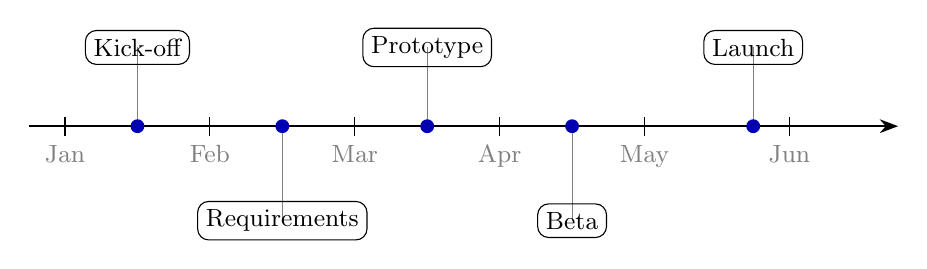
\begin{tikzpicture}[
  x=0.92cm,
  every node/.style={font=\small},
  milestone/.style={draw, rounded corners, inner sep=3pt},
]
  \draw[thick, -{Stealth}] (0,0) -- (12,0);
  \foreach \x/\month in {0.5/Jan, 2.5/Feb, 4.5/Mar, 6.5/Apr, 8.5/May, 10.5/Jun}
    \draw (\x,0.12) -- (\x,-0.12) node[below, gray] {\month};
  \foreach \x/\y/\event in {1.5/1/Kick-off, 3.5/-1.2/Requirements, 5.5/1/Prototype, 7.5/-1.2/Beta, 10/1/Launch} {
    \draw[gray] (\x,0) -- (\x,\y);
    \fill[blue!70!black] (\x,0) circle (2.5pt);
    \node[milestone] at (\x,\y) {\event};
  }
\end{tikzpicture}
